\documentclass[../../main/main.tex]{subfiles}
\graphicspath{{./figures/}}

\dominitoc
\faketableofcontents

% \renewcommand{\mtcSfont}{\small\bfseries}
% \renewcommand{\mtcSSfont}{\footnotesize}

\makeatletter
\renewcommand{\@chapapp}{Chimie -- chapitre}
\makeatother

% \toggletrue{student}
% \toggletrue{corrige}
% \renewcommand{\mycol}{black}
% \renewcommand{\mycol}{gray}

\hfuzz=5.002pt

\begin{document}
\setcounter{chapter}{4}

\settype{prof}
\settype{stud}
\settype{book}

\chapter{R\'eactions de précipitation}

\vspace*{\fill}

\begin{prgm}
	% \footnotesize
	\begin{tcb}*(ror)"know"{Savoirs}
		\begin{itemize}
			\item Constante de l'équation de dissolution, produit de solubilité $K_s$
			\item Solubilité et condition de précipitation, domaine d'existence,
			      facteurs influençant la solubilité.
		\end{itemize}
	\end{tcb}
	\begin{tcb}*(ror)"how"{Savoir-faire}
		\begin{itemize}
			\item Déterminer la valeur de la constante d'équilibre pour une équation
			      de réaction, combinaison linéaire d'équations dont les constantes
			      thermodynamiques sont connues.
			\item Déterminer la composition chimique du système dans l'état final, en
			      distinguant les cas d'équilibre chimique et de transformation totale,
			      pour une transformation modélisée par une réaction chimique unique.
			\item Prévoir l'état de saturation ou de non saturation d'une solution.
			\item Utiliser les diagrammes de prédominance ou d'existence pour prévoir
			      les espèces incompatibles ou la nature des espèces majoritaires.
			\item Exploiter les courbes d'évolution de la solubilité d'un solide en
			      fonction d'une variable.
			\item Illustrer un procédé de retraitement, de recyclage, de séparation
			      en solution aqueuse.
		\end{itemize}
	\end{tcb}
\end{prgm}

\vspace*{\fill}
\minitoc
\vspace*{\fill}

\newpage

\vspace*{\fill}
% {
\begin{boxes}
	% \footnotesize
	\begin{tcb}(defi)<lftt>{Liste des définitions}
		\tcblistof[\paragraph*]{defi}{\hspace*{6pt}}
	\end{tcb}
	\begin{tcb}(rapp)<lftt>{Liste des rappels}
		\tcblistof[\paragraph*]{rapp}{\hspace*{6pt}}
	\end{tcb}
	\begin{tcb}(prop)<lftt>{Liste des propriétés}
		\tcblistof[\paragraph*]{prop}{\hspace*{6pt}}
		% \tcblistof[\paragraph*]{loi}{\hspace*{6pt}}
		\tcblistof[\paragraph*]{theo}{\hspace*{6pt}}
	\end{tcb}
	% \begin{tcb}(coro)<lftt>{Liste des corollaires}
	% 	\tcblistof[\paragraph*]{coro}{\hspace*{6pt}}
	% \end{tcb}
	% \begin{tcb}(demo)<lftt>{Liste des démonstrations}
	% 	\tcblistof[\paragraph*]{demo}{\hspace*{6pt}}
	% 	\tcblistof[\paragraph*]{prev}{\hspace*{6pt}}
	% \end{tcb}
	% \begin{tcb}(inte)<lftt>{Liste des interprétations}
	% 	\tcblistof[\paragraph*]{inte}{\hspace*{6pt}}
	% \end{tcb}
	% \begin{tcb}(tool)<lftt>{Liste des outils}
	% 	\tcblistof[\paragraph*]{tool}{\hspace*{6pt}}
	% \end{tcb}
	% \begin{tcb}(nota)<lftt>{Liste des notations}
	% 	\tcblistof[\paragraph*]{nota}{\hspace*{6pt}}
	% \end{tcb}
	\begin{tcb}(appl)<lftt>{Liste des applications}
		\tcblistof[\paragraph*]{appl}{\hspace*{6pt}}
	\end{tcb}
	\begin{tcb}(rema)<lftt>{Liste des remarques}
		\tcblistof[\paragraph*]{rema}{\hspace*{6pt}}
	\end{tcb}
	\begin{tcb}(exem)<lftt>{Liste des exemples}
		\tcblistof[\paragraph*]{exem}{\hspace*{6pt}}
	\end{tcb}
	\begin{tcb}(ror)<lftt>{Liste des points importants}
		\tcblistof[\paragraph*]{ror}{\hspace*{6pt}}
	\end{tcb}
	\begin{tcb}(impo)<lftt>{Liste des erreurs communes}
		\tcblistof[\paragraph*]{impo}{\hspace*{6pt}}
	\end{tcb}
\end{boxes}
% }
\vspace*{\fill}
\newpage

\section{Équilibre d'un solide en solution}

\subsection{Dissolution et précipitation}
\begin{tcb*}(rapp){Dissolution}
	Une espèce solide $\ce{X\sol}$ est capable d'être dissoute, c'est-à-dire passer
	en solution\ftn{Dans notre cas, le solvant sera toujours l'eau.}~:
	\psw{
		\[
			\ce{A_pB_q\sol{}} = p \ce{A+}\aqu{} + q \ce{B-}\aqu
		\]
	}
	\vspace{-15pt}
\end{tcb*}

\begin{tcb*}(rema)<lftt>{Solides usuels}
	\begin{itemize}
		\item Le plus souvent, le solide se décompose en ions, et ce sont ces
		      derniers qui seront solvatés.
		\item Chimiquement, la dissolution consiste en la séparation des molécules
		      de \ce{X} par le solvant, grâce aux interactions moléculaires~:
		      \begin{center}
			      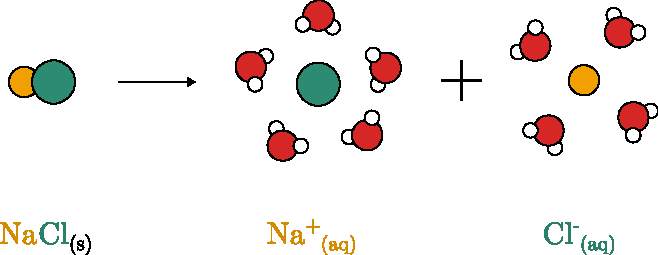
\includegraphics[scale=.8]{dissolution}
		      \end{center}
	\end{itemize}
\end{tcb*}

\begin{tcb*}[sidebyside, righthand ratio=.3](defi){Solubilité}
	Un solide ne pourra souvent pas se dissoudre totalement dans l'eau, et il y
	aura à un moment une \textbf{saturation}. On appelle alors \textbf{solubilité}
	la \textbf{concentration maximale d'espèce dissoute}~:
	\psw{
		\[
			\boxed{s = \frac{n\ind{dis,max}}{V}}
		\]
	}
	\vspace{-15pt}
	\tcblower
	\tcbsubtitle{\fatbox{\textbf{Unité}}}
	\psw{
		\[
			\si{mol.L^{-1}}
		\]
	}
\end{tcb*}

\begin{tcb*}(rema)<lftt>{Solubilités tabulées}
	Souvent, les données tabulées utilisent le \si{g.mol^{-1}}. Pour passer de
	l'une à l'autre, il faut simplement convertir grâce à ~:
	\psw{
		\[
			m\ind{dissout} = M n\ind{dissout}
		\]
	}
	\vspace{-15pt}
\end{tcb*}

\begin{tcb*}(exem)<lftt>{Solubilités usuelles}
	\begin{center}
		\captionof{table}{Solubilités de quelques solides dans l'eau}
		\begin{tabular}{cc}
			\toprule
			\textbf{Solide} & \textbf{Solubilité} (\si{g.mol^{-1}})
			\\
			\midrule
			\ce{NaCl} (sel) & \num{357}
			\\
			Saccharose      & \num{2000}
			\\
			$\ce{O2\gaz}$   & \num{1120}
			\\
			\bottomrule
		\end{tabular}
	\end{center}
\end{tcb*}

\begin{tcb*}(defi){Précipité et précipitation}
	Un précipité est un \textbf{dépôt solide} en \textbf{équilibre} avec la phase
	aqueuse, qui apparaît lorsqu'une solution est \textbf{saturée} en composés
	ionique ou moléculaire.
	\smallbreak
	On appelle \textbf{précipitation} la réaction de formation du solide à partir
	de ses composés ioniques~:
	\psw{
		\[
			p \ce{A+}\aqu{} + q \ce{B-}\aqu{} = \ce{A_pB_q\sol{}}
		\]
	}
	\vspace{-15pt}
\end{tcb*}

\begin{tcb*}(expe){Précipitation d'hydroxyde de cuivre}
	\begin{center}
		\url{https://www.youtube.com/watch?v=G-o2zF1Kbxo}
	\end{center}
	Lorsque l'on ajoute de la soude $(\ce{Na+},\ce{HO-})$ à une solution de sulfate
	de cuivre $(\ce{Cu^2+},\ce{SO_4^2-})$, un précipité solide d'hydroxyde de cuivre
	\ce{Cu(OH)2} apparaît. On peut le filtrer et l'isoler.
	\smallbreak
	On retrouve cette situation
	pour beaucoup d'autres solutions, avec de nombreux précipités~: \ce{AgCl},
	\ce{Zn(OH)2}, etc.
\end{tcb*}

Il y a deux façons d'obtenir un précipité~:
\begin{enumerate}
	\bitem{En introduisant un excès de solide dans l'eau}~: si on dissout du sel
	dans l'eau, passé une certain quantité le sel ne se dissout plus~: il reste
	du solide au fond de la solution~;
	\bitem{En mélangeant deux solutions contenant les espèces constituantes du
		précipité}~: c'est le cas de l'expérience présentée.
\end{enumerate}

\subsection{Équilibre}
\begin{tcb*}(defi){Produit de solubilité}
	Le produit de solubilité est la constante d'équilibre de la \textbf{réaction
		de dissolution}, noté $K_s$. Par exemple~:
	\vspace{-15pt}
	\psw{
		\begin{gather*}
			\ce{AgCl\sol{} = Ag+\aqu{} + Cl^-\aqu{}}
			\tag*{$K_s$}
			\\
			\beforetext{Avec}
			\boxed{
				K_s = \frac{[\ce{Ag+}]\ind{eq}\times
					[\ce{Cl-}]\ind{eq}}{{c^\circ}^2}
			}
		\end{gather*}
	}
	On définira également $\pk[s] = - \log K_s$.
\end{tcb*}

\begin{tcb*}[cnt,bld](impo){Produit de solubilité}
	Le produit de solubilité est associé à la réaction de \xul{dissolution}~!
\end{tcb*}

\begin{tcb*}(ror){Méthode pour calculer une solubilité}
	\begin{enumerate}[label=\sqenumi]
		\item Écrire la réaction \textbf{de dissolution} et dresser le tableau
		      d'avancement en \textbf{supposant la saturation}~;
		\item Exprimer $s$ en fonction de $\xi\ind{eq}$ puis
		      les \textbf{concentrations en fonction de $s$}~;
		\item Exprimer $K_s$ en fonction de $s$ et résoudre.
	\end{enumerate}
\end{tcb*}

\begin{tcb*}[breakable, label=appl:calcsol](appl)<lftt>{Calcul de solubilité}
	Calculer la solubilité en \si{mol.L^{-1}} puis en \si{g.L^{-1}}pour les
	espèces suivantes~:
	\begin{enumerate}
		\item $\ce{NaCl\sol}$ de $K_s = \num{36}$ avec $M_{\ce{NaCl}} =
			      \SI{58.44}{g.mol^{-1}}$~;
		\item $\ce{PbI_2\sol}$ de $\pk[s] = \num{7.5}$ avec $M_{\ce{PbI_2}} =
			      \SI{461.01}{g.mol^{-1}}$.
	\end{enumerate}
	\tcblower
	\newpage
	\begin{enumerate}
		\item
		      \begin{enumerate}[label=\sqenumi]
			      \item ~
			            \vspace{-23pt}
			            \begin{center}
				            \def\rhgt{0.50}
				            \centering
				            \begin{tabularx}{\linewidth}{|l|c||YdYdY|}
					            \hline
					            \multicolumn{2}{|c||}{
						            $\xmathstrut{\rhgt}$
					            \textbf{Équation}}     &
					            \psw{$\ce{NaCl\sol}$}  & $=$                        &
					            \psw{$\ce{Na+\aqu}$}   & $+$                        &
					            \psw{$\ce{Cl^-\aqu}$}                                 \\
					            \hline
					            $\xmathstrut{\rhgt}$
					            Initial                & $\xi = 0$                  &
					            \psw{$n$}              & \vline                     &
					            \psw{$0$}              & \vline                     &
					            \psw{$0$}                                             \\
					            \hline
					            $\xmathstrut{\rhgt}$
					            Final                  & $\xi_f = \psw{\xi_{\equ}}$ &
					            \psw{$n - \xi_{\equ}$} & \vline                     &
					            \psw{$\xi_{\equ}$}     & \vline                     &
					            \psw{$\xi_{\equ}$}                                    \\
					            \hline
				            \end{tabularx}
			            \end{center}
			      \item \leavevmode\vspace*{-33pt}\relax
			            \psw{
				            \begin{gather*}
					            \beforetext{Par définition,}
					            n\ind{dis,max} = \xi\ind{eq} = sV
					            \quad \Ra \quad
					            \left\{
					            \begin{array}{rl}
						            [\ce{Na+}]\ind{eq} & = s
						            \\{}
						            [\ce{Cl-}]\ind{eq} & = s
					            \end{array}
					            \right.
				            \end{gather*}
			            }
			      \item \leavevmode\vspace*{-33pt}\relax
			            \psw{
				            \begin{gather*}
					            \beforetext{Or,}
					            K_s =
					            \frac{[\ce{Na+}]\ind{eq}\times[\ce{Cl-}]\ind{eq}}{{c^\circ}^2} =
					            \left( \frac{s}{c^\circ} \right)^2
					            \\\Ra
					            \boxed{s = c^\circ \sqrt{K_s}}
					            \quad \Ra \quad
					            \xul{s = \SI{6}{mol.L^{-1}} = \SI{350}{g.L^{-1}}}
				            \end{gather*}
			            }
		      \end{enumerate}
		\item
		      \begin{enumerate}[label=\sqenumi]
			      \item ~
			            \vspace{-23pt}
			            \begin{center}
				            \def\rhgt{0.50}
				            \centering
				            \begin{tabularx}{\linewidth}{|l|c||YdYdY|}
					            \hline
					            \multicolumn{2}{|c||}{
						            $\xmathstrut{\rhgt}$
					            \textbf{Équation}}       &
					            \psw{$\ce{PbI_2\sol}$}   & $=$                  &
					            \psw{$\ce{Pb^{2+}\aqu}$} & $+$                  &
					            \psw{$2\ce{I^-\aqu}$}                             \\
					            \hline
					            $\xmathstrut{\rhgt}$
					            Initial                  & $\xi = 0$            &
					            \psw{$n$}                & \vline               &
					            \psw{$0$}                & \vline               &
					            \psw{$0$}                                         \\
					            \hline
					            $\xmathstrut{\rhgt}$
					            Final                    & $\xi_f = \xi_{\equ}$ &
					            \psw{$n - \xi_{\equ}$}   & \vline               &
					            \psw{$\xi_{\equ}$}       & \vline               &
					            \psw{$2\xi_{\equ}$}                               \\
					            \hline
				            \end{tabularx}
			            \end{center}
			      \item \leavevmode\vspace*{-33pt}\relax
			            \psw{
				            \begin{gather*}
					            \beforetext{Par définition,}
					            n\ind{dis,max} = \xi\ind{eq} = sV
					            \quad \Ra \quad
					            \left\{
					            \begin{array}{rl}
						            [\ce{Pb^2+}]\ind{eq} & = s
						            \\{}
						            [\ce{I-}]\ind{eq}    & = 2s
					            \end{array}
					            \right.
				            \end{gather*}
			            }
			      \item \leavevmode\vspace*{-35pt}\relax
			            \psw{
				            \begin{gather*}
					            \beforetext{Or,}
					            K_s =
					            \frac{[\ce{Pb^2+}]\ind{eq}\times[\ce{I-}]^2\ind{eq}}{{c^\circ}^3} =
					            4\left( \frac{s}{c^\circ} \right)^3
					            \\\Ra
					            \boxed{s = c^\circ \left( \frac{10^{-\pk[s]}}{4} \right)^{1/3}}
					            \quad \Ra \quad
					            \xul{s = \SI{2.0e-3}{mol.L^{-1}} = \SI{0.92}{g.mol^{-1}}}
				            \end{gather*}
			            }
		      \end{enumerate}
	\end{enumerate}
	\vspace{-15pt}
\end{tcb*}

\subsection{Condition d'existence d'un précipité}
\begin{tcb*}(rapp){Sens d'évolution d'un système}
	\begin{center}
		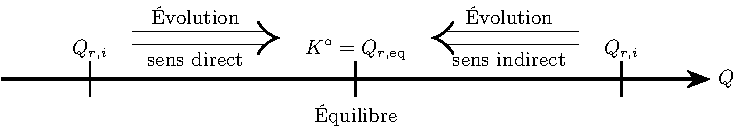
\includegraphics[scale=1]{QKequi}
	\end{center}
\end{tcb*}

\begin{tcb*}[breakable, label=appl:prenon](appl)<lftt>{Précipitation ou non~?}
	On ajoute $n = \SI{e-5}{mol}$ d'ions \ce{Cl-} dans $V_0 = \SI{10}{mL}$ de
	nitrate d'argent $\left( \ce{Ag+},\ce{NO_3^-} \right)$ à $c_0 =
		\SI{e-3}{mol.L^{-1}}$. On donne $\pk[s](\ce{AgCl}) = \num{9.8}$.
	\begin{center}
		\fbox{\textbf{Obtient-on un précipité de chlorure d'argent \ce{AgCl}~?}}
	\end{center}
	\tcblower
	\psw{
		La réaction de formation de \ce{AgCl} est
		\begin{gather*}
			\ce{Ag+\aqu{} + Cl^-\aqu{} = AgCl\sol{} }
			\tag*{$K^\circ = \frac{1}{K_s}$}
		\end{gather*}
	}
	\vspace*{-20pt}
	\psw{
		\begin{gather*}
			\beforetext{Sens direct $\Ra$}
			Q_{r,i} < \frac{1}{K_s}
			\Lra
			\frac{{c^\circ}^2}{[\ce{Ag+}]_i[\ce{Cl-}]_i} < \frac{1}{K_s}
			\Lra
			\boxed{\frac{[\ce{Ag+}]_i[\ce{Cl-}]_i}{{c^\circ}^2} > K_s}
			\\\AN
			[\ce{Ag+}]_i = \SI{e-3}{mol.L^{-1}}
			\qet
			[\ce{Cl-}]_i = n/V_0 = \SI{e-3}{mol.L^{-1}}
			\quad \Ra \quad
			\xul{[\ce{Ag+}]_i[\ce{Cl-}]_i = \num{e-6} > K_s}
		\end{gather*}
		Il y a donc bien formation du précipité.
	}
\end{tcb*}

%[sidebyside, sidebyside align=top]
\begin{tcb*}[breakable](prop){Condition d'existence d'un précipité}
	\begin{itemize}
		\item
		      \leftcentersright{%
			      \textbf{Dissolution}~:
		      }{
			      $\ce{A_pB_q\sol{}} = p \ce{A+}\aqu{} + q \ce{B-}\aqu$
		      }{%
			      $K_s$
		      }
	\end{itemize}
	\vspace{-15pt}
	\begin{isd}
		\begin{itemize}[label=$\triangleright$]
			\bitem{Solide = équilibre = saturation}
			\smallbreak
			$\Lra$ suffisamment de solide initial
			\psw{
				\[
					Q_{r,f}\sup{dis} = Q_{r,\equ} = K_s
				\]
			}
			\vspace{-15pt}
		\end{itemize}
		\tcblower
		\begin{itemize}[label=$\triangleright$]
			\bitem{Pas de solide = pas d'équilibre}
			\smallbreak
			$\Lra$ solide totalement dissout
			\psw{
				\[
					Q_{r,f}\sup{dis} < K_s
				\]
			}
			\vspace{-15pt}
		\end{itemize}
	\end{isd}
	\tcblower
	\begin{itemize}
		\item
		      \leftcentersright{%
		      \textbf{Précipitation}~:
		      }{
		      $p \ce{A+}\aqu{} + q \ce{B-}\aqu{} = \ce{A_pB_q\sol{}}$
		      }{%
		      $K^\circ = \psw{K_s{}^{-1}}$
		      }
	\end{itemize}
	\vspace{-15pt}
	\begin{isd}
		\begin{itemize}[label=$\triangleright$]
			\bitem{Solide = équilibre}
			\smallbreak
			$\Lra$ suffisamment d'ions
			\psw{
			\[
				\frac{[\ce{A+}]_i{}^p [\ce{B-}]_i{}^q}{(c^\circ)^{p+q}} > K_s
				\qet
				Q_{r,f}\sup{pre} = Q_{r,\equ}\sup{pre} = K^\circ
			\]
			}
			\vspace{-15pt}
		\end{itemize}
		\tcblower
		\begin{itemize}[label=$\triangleright$]
			\bitem{Pas de solide = pas d'équilibre}
			\smallbreak
			$\Lra$ pas assez d'ions
			\psw{
			\[
				Q_{r,i}\sup{pre} > K^\circ
				\Lra
				\frac{[\ce{A+}]_i{}^p [\ce{B-}]_i{}^q}{(c^\circ)^{p+q}} < K_s
			\]
			}
			\vspace{-15pt}
		\end{itemize}
	\end{isd}
\end{tcb*}

\begin{tcb*}(exem)<lftt>{Rupture d'équilibre de dissolution}
	En reprenant l'application~\ref{appl:calcsol}, s'il n'y a pas de solide ça
	veut dire qu'il a été entièrement consommé~; alors,
	\psw{
		\begin{gather*}
			\xi_f = \xi\ind{max} = n < \xi\ind{eq}
			\Lra
			Q_{r,f} = \frac{[\ce{Ag+}]_f\times[\ce{Cl-}]_f}{{c^\circ}^2} <
			\frac{[\ce{Ag+}]\ind{eq}\times[\ce{Cl-}]\ind{eq}}{{c^\circ}^2} = K_s
			\Lra
			\boxed{Q_{r,f} < K_s}
			\qed
		\end{gather*}
	}
	\vspace{-15pt}
\end{tcb*}

\begin{tcb*}(ror){Diagramme d'existence d'un solide}
	Pour un solide, soit il existe soit il n'existe pas~: on ne parle pas de
	prédominance mais d'existence. La construction d'un tel diagramme reflète ce
	qui a été déterminé plus tôt~:
	\begin{center}
		\textbf{\fbox{Un précipité existe si la solution est chargée en ions}}
	\end{center}
	On trace donc les domaines d'un solide \ce{A_pB_q} en fonction de la
	concentration d'un de ses ions \textit{via} $\prm \ce{A}$ ou $\prm \ce{B}$.
	\begin{center}
		\sswitch{
			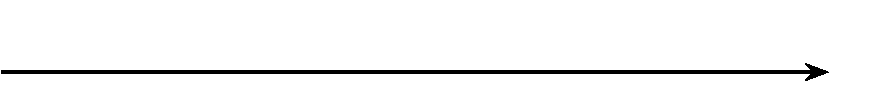
\includegraphics[scale=1]{exist_plain}
		}{
			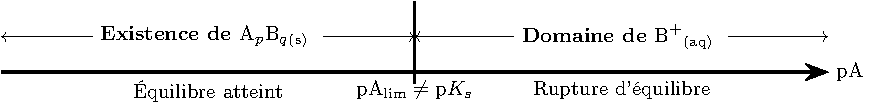
\includegraphics[scale=1]{existA}
		}
		\captionof{figure}{Diagramme d'existence générique}
	\end{center}
	\textbf{Méthode}~:
	On détermine le $\prm \ce{A}\ind{lim}$ d’apparition du solide en se plaçant à
	la \textbf{limite de la précipitation}~: on suppose que la première molécule
	de solide vient d’apparaitre, donc l’équilibre $Q\ind{eq} = K_s$ est vérifié,
	mais les concentrations des ions ne sont pas modifiées par la précipitation.
\end{tcb*}

\begin{tcb*}(appl)<lftt>{Diagramme d'existence \ce{AgCl}}
	Tracer le diagramme d'existence de $\ce{AgCl\sol{}}$ en fonction de $\prm
		\ce{Cl}$, pour une solution de \ce{Ag+} à $c_0 = \SI{0.10}{mol.L^{-1}}$.
	\tcblower
	On reprend le résultat de l'application~\ref{appl:prenon} avec $[\ce{Ag+}]_i =
		c_0$~:
	\psw{
		\begin{gather*}
			\frac{[\ce{Ag+}]_i[\ce{Cl-}]_i}{{c^\circ}^2} > K_s
			\Lra
			\frac{[\ce{Cl-}]_i}{c^\circ} > \frac{K_s}{c_0}c^\circ
			\Lra
			\boxed{\prm \ce{Cl} < \pk[s] + \log (c_0)}
			\Ra \AN
			\xul{\prm \ce{Cl}\ind{lim} = \num{8.8}}
		\end{gather*}
	}
	\vspace{-15pt}
	\begin{center}
		\sswitch{
			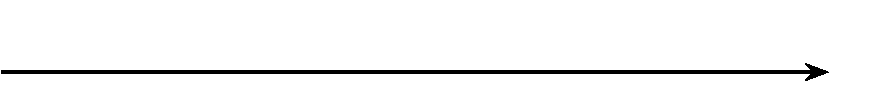
\includegraphics[scale=1]{exist_plain}
		}{
			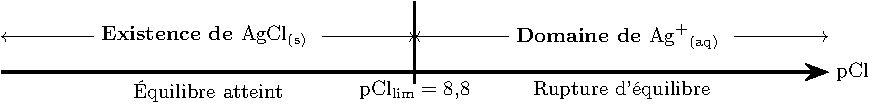
\includegraphics[scale=1]{exist_AgCl-Cl}
		}
		\captionof{figure}{Diagramme d'existence de \ce{AgCl}}
	\end{center}
\end{tcb*}

\section{Facteurs influençant la solubilité}
\subsection{Température}

\begin{tcb*}(prop){Influence de la température}
	La solubilité dépend de la température car le produit de solubilté dépend de
	la température ($K_s(T)$). La plupart du temps, \textbf{la solubilité
		augmente\ftn{Contre-exemple~: le calcaire.} avec $T$}
\end{tcb*}
\begin{tcb*}(exem)<lftt>{Utilistion pratique}
	On peut se servir de cette propriété à des fins de purification.
	Supposons que l'on dispose
	d'un mélange d'un composé A avec une impureté B dont on veut se débarasser. Si
	on trouve un solvant dans lequel \xul{les impuretés sont plus solubles} que le composé
	principal, on peut réaliser une \textbf{recristallisation}~:
	\begin{enumerate}
		\item On dissout le mélange
		      dans la plus petite quantité de \textbf{solvant chaud} pour bien dissoudre
		      le mélange, apportant ainsi une solution \textbf{saturée}~;
		\item La solution est ensuite laissée à refroidir~;
		\item Comme la solution refroidit, la solubilité des composés
		      diminue, et le composé désiré cristallise tandis que les impuretés restent en
		      solution.
	\end{enumerate}
\end{tcb*}

\subsection{Effet d'ions communs}
\begin{tcb*}(prop){Effet d'ions communs}
	Lors d'une dissolution, si la solution contient déjà l'un des ions du solide
	alors la saturation appraît plus tôt~: \textbf{la solubilité diminue}.
\end{tcb*}
\begin{tcb*}[breakable](appl)<lftt>{Effet d'ions communs sur $\ce{AgCl\sol}$}
	Calculer la solubilité de $\ce{AgCl\sol}$ s'il y a déjà $c =
		\SI{0.1}{mol.L^{-1}}$ de \ce{Cl-} en solution et comparer la solubilité
	obtenue au résultat attendu sans. On donne $\pk[s](\ce{AgCl}) = \num{9.75}$.
	\tcblower
	\begin{enumerate}[label=\sqenumi]
		\item \leavevmode\vspace*{-30pt}\relax
		      \begin{center}
			      \def\rhgt{0.50}
			      \centering
			      \begin{tabularx}{\linewidth}{|l|c||YdYdY|}
				      \hline
				      \multicolumn{2}{|c||}{
					      $\xmathstrut{\rhgt}$
				      \textbf{Équation}}     &
				      \psw{$\ce{AgCl\sol}$}  & $=$                        &
				      \psw{$\ce{Ag+\aqu}$}   & $+$                        &
				      \psw{$\ce{Cl^-\aqu}$}                                 \\
				      \hline
				      $\xmathstrut{\rhgt}$
				      Initial                & $\xi = 0$                  &
				      \psw{$n$}              & \vline                     &
				      \psw{$0$}              & \vline                     &
				      \psw{$cV$}                                            \\
				      \hline
				      $\xmathstrut{\rhgt}$
				      Final                  & $\xi_f = \psw{\xi_{\equ}}$ &
				      \psw{$n - \xi_{\equ}$} & \vline                     &
				      \psw{$\xi_{\equ}$}     & \vline                     &
				      \psw{$cV + \xi_{\equ}$}                               \\
				      \hline
			      \end{tabularx}
		      \end{center}
		\item \leavevmode\vspace*{-33pt}\relax
		      \psw{
			      \begin{gather*}
				      \beforetext{Par définition,}
				      n\ind{dis,max} = \xi\ind{eq} = sV
				      \quad \Ra \quad
				      \left\{
				      \begin{array}{rl}
					      [\ce{Ag+}]\ind{eq} & = s
					      \\{}
					      [\ce{Cl-}]\ind{eq} & = \frac{cV + \xi\ind{eq}}{V} = c+s
				      \end{array}
				      \right.
			      \end{gather*}
		      }
		\item \leavevmode\vspace*{-33pt}\relax
		      \psw{
			      \begin{gather*}
				      \beforetext{Or,}
				      K_s =
				      \frac{[\ce{Ag+}]\ind{eq}\times[\ce{Cl-}]\ind{eq}}{{c^\circ}^2} =
				      \frac{s(c+s)}{(c^\circ)^2}
				      \\\Ra
				      \beforetext{On suppose $s \ll \SI{0.1}{mol.L^{-1}}$}
				      s \times c \approx  K_s
				      \Lra
				      \boxed{s \approx \frac{K_s}{c}}
				      \\\Ra
				      \xul{s = \SI{1.8e-9}{mol.L^{-1}}}
			      \end{gather*}
		      }
		      \vspace{-15pt}
	\end{enumerate}
	\vspace{-15pt}
\end{tcb*}

\subsection{Influence du pH}
\begin{tcb*}(prop){Influence du pH}
	Lorsque les espèces en jeu appartiennt en plus à un couple acide-base, le pH a
	rôle sur la solubilité~:
	\begin{itemize}
		\item Un solide \textbf{basique} aura une plus grande solubilité en
		      \textbf{milieu acide}~;
		\item Un solide acide aura une plus grande solubilité en milieu basique.
	\end{itemize}
\end{tcb*}
\begin{tcb*}(exem)<lftt>{Dissolution d'oxyde d'aluminium en fonction du pH}
	$\ce{Al(OH)3\sol}$ appartient au coule acide-base
	\[
		\red{\ce{Al(OH)3\sol}}/\blu{\ce{Al(OH)4^-\aqu}}
	\]
	Étudions sa dissolution dans l'eau~:
	\smallbreak
	\noindent
	\begin{minipage}[c]{.69\linewidth}
		\begin{center}
			\def\rhgt{0.50}
			\centering
			\begin{tabularx}{\linewidth}{|c||YdYdYdY|}
				\hline
				$\xmathstrut{\rhgt}$ \textbf{Équation} &
				\psw{$\ce{Al(OH)3\sol}$}               & $+$    &
				\psw{$\ce{H_2O\liq}$}                  & $\ra$  &
				\psw{$\ce{Al(OH)4^-\aqu}$}             & $+$    &
				\psw{$\ce{H+\aqu}$}                               \\
				\hline
				$\xmathstrut{\rhgt}$
				$\xi = 0$                              &
				\psw{$n$}                              & \vline &
				\psw{excès}                            & \vline &
				\psw{$0$}                              & \vline &
				\psw{$[\ce{H+}]_0V$}                              \\
				\hline
				$\xmathstrut{\rhgt}$
				$\xi_{\equ} = \psw{sV}$                &
				\psw{$n - sV$}                         & \vline &
				\psw{excès}                            & \vline &
				\psw{$sV$}                             & \vline &
				\psw{$[\ce{H+}]V$}                                \\
				\hline
			\end{tabularx}
		\end{center}
		\vspace{-15pt}
		\psw{
			\begin{gather*}
				\beforetext{D'où}
				K_s = \frac{s \pa{s+[\ce{H+}]_0}}{{c^\circ}^2} = \frac{s[\ce{H+}]}{{c^\circ}^2}
				\\\Ra
				\pk[s] = \pH + \prm s
				\Lra
				\boxed{\prm s = \pk[s] - \pH}
			\end{gather*}
		}
	\end{minipage}
	\hfill
	\begin{minipage}[c]{.30\linewidth}
		\begin{center}
			\sswitch{
				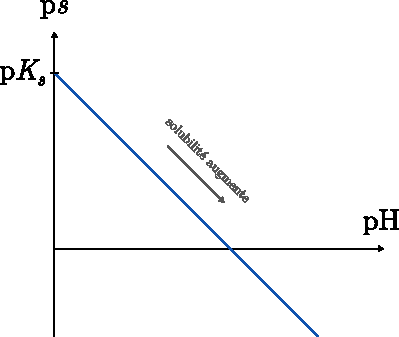
\includegraphics[width=\linewidth, draft=true]{psph}
			}{
				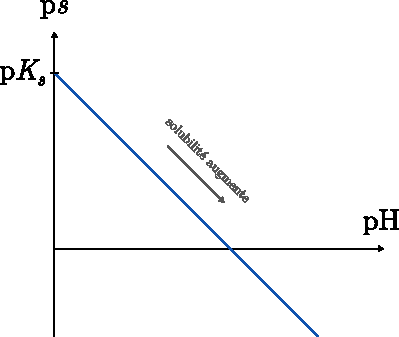
\includegraphics[width=\linewidth]{psph}
			}
			\captionof{figure}{Graph $\prm s$-$\pH$}
		\end{center}
	\end{minipage}
\end{tcb*}

\end{document}
